\documentclass[11pt]{article}
\usepackage[margin=2.2cm]{geometry}
\usepackage{amsmath,amssymb}
\usepackage{graphicx}
\usepackage{booktabs}
\usepackage{longtable}
\usepackage{xcolor}
\usepackage{hyperref}
\usepackage{caption}
\usepackage{float}
\usepackage[htt]{hyphenat}
\usepackage{enumitem}

\emergencystretch=3em
\sloppy
\setlength{\tabcolsep}{4.5pt}

\newcommand{\Q}{\mathbb Q}
\newcommand{\Pp}{\mathbb P}
\newcommand{\E}{\mathbb E}
\newcommand{\R}{\mathbb R}

\title{The explicit DLV $\times$ extended-Bates CRC construction:\\
implementation, audit, and verification against\\
the DYSANOS~II manuscript's own synthetic reset sequence}
\author{\texttt{quant\_data-main/quantdata/dysanos/bates\_crc}}
\date{\today}

\begin{document}
\maketitle

\begin{abstract}
We implement the explicit DLV $\times$ extended-Bates construction
(\texttt{thm:dlv-bates}), the off-grid drift corollary
(\texttt{cor:bates-offgrid-drift}), and Section~12's branching lemma,
reserve theorem, and synthetic reset sequence, from the current DYSANOS~II
manuscript, using theorem labels and content rather than page numbers. The
Heston Riccati coefficient and Gaussian Bates jump exponent are re-derived
in closed form and checked against an independent RK4 ODE integration and
an independent Gauss--Hermite quadrature respectively. The Section~12
reserve mechanism is checked against the manuscript's own fully-specified
synthetic reset sequence, reproducing its $\theta$-path and reserve-usage
column exactly. The branching lemma's L\'evy-measure positivity claim is
established analytically (via Sato's convolution-semigroup theorem and the
classical Duffie--Filipovic--Schachermayer affine-admissibility criterion),
explicitly \emph{not} via a numerical frequency sweep, per the task's own
instruction. A coherent finite-state latent DLV factor is connected to the
reserve-CRC Bates factor via the manuscript's finite-mixture pricing
formula, and its positivity/tower/settlement properties are verified before
any connection to a trained decoder is attempted. A verification battery
establishes, to machine precision, the central and previously-unverified
claim of the whole construction: options settling before a scheduled reset
are exactly price-invariant across that reset, while longer-dated options
are (by design) not -- confirmed further by a negative control that
violates this invariance when the reserve mechanism is removed. This task
runs entirely without market data, as instructed.
\end{abstract}

\tableofcontents

\section{Executive summary}
\label{sec:exec}

\begin{enumerate}
\item \textbf{Audit first} (Sec.~\ref{sec:audit-summary}, full detail in
  \texttt{AUDIT.md}): every claim below was checked against the running
  code, not asserted from the manuscript. The audit surfaces one
  significant, non-obvious structural finding (the current local jump
  parameters $p_n$ cancel out of the priced dynamics exactly) and is
  explicit about what remains unverifiable without data ($X$/$Y$
  independence, full product martingality).
\item \textbf{Background machinery} (Sec.~\ref{sec:background}): the
  Riccati/jump-exponent/continuation-transform stack is closed-form,
  independently cross-checked, and its martingale normalisation is proven
  analytically and confirmed numerically for the full assembled transform.
\item \textbf{Reserve CRC} (Sec.~\ref{sec:reserve}): the exact reset
  mechanics reproduce the manuscript's own synthetic sequence table to
  $<10^{-12}$; the branching lemma is proven analytically, with the
  admissibility of the reserve term itself reducing to a nonnegativity
  invariant already enforced in code.
\item \textbf{Coherent latent DLV product} (Sec.~\ref{sec:dlv-product}): a
  verified finite-state martingale chain is connected to the Bates factor;
  mass, tower, and settlement properties are confirmed before any
  connection to a trained decoder.
\item \textbf{Verification battery} (Sec.~\ref{sec:verification}): the
  central ``protected options are exactly reset-invariant'' claim is
  confirmed to machine precision across every scheduled reset and an
  independent strike mesh, and is shown (via a negative control) to be a
  real, non-vacuous property of the reserve mechanism.
\item \textbf{What remains open} (Sec.~\ref{sec:deferred}): $X$/$Y$
  independence and full product martingality are modelling assumptions
  that cannot be checked without market data; connection to a trained
  Wiese--Wissel decoder is correctly scoped as the next step.
\end{enumerate}

\section{Audit before claiming exactness}
\label{sec:audit-summary}

The full audit (true martingality, conditional independence, terminal
settlement, finite horizon, L\'evy integrability, jump-compensation
convention, the Heston branching argument, and a non-obvious structural
finding about how $p_n$ enters the priced dynamics) is written up in full
in \texttt{AUDIT.md}, produced \emph{before} any exactness claim was made
elsewhere in this report. Its summary table is reproduced here.

\begin{center}
\small
\begin{tabular}{ll}
\toprule
Item & Status \\
\midrule
$D(-i,\tau)=A(-i,\tau)=0$ for all $\tau$ & PROVEN + VERIFIED \\
$j_p(0)=j_p(-i)=0$ & PROVEN + VERIFIED (incl.\ independent quadrature) \\
Full transform $\Phi(0)=\Phi(-i)=1$ & VERIFIED ($<10^{-8}$) \\
Manuscript's synthetic reset sequence reproduced & VERIFIED ($<10^{-12}$, exact table match) \\
Envelope dominates every box member & VERIFIED (grid + closed-form bound) \\
Branching lemma $D(u,r)$ positivity & PROVEN analytically (Sato) -- not by sweep \\
Reserve-term admissibility ($\kappa b_{\rm used}\ge0$) & PROVEN (DFS 2003) + enforced as code invariant \\
$p_n$ cancels out of priced dynamics & VERIFIED, non-obvious, documented \\
Independent MC pricing check & VERIFIED, pre-first-reset window \\
Protected-option ($T<t_n$) exact invariance & VERIFIED ($<10^{-8}$, 48 combinations) \\
Negative control violates invariance & VERIFIED ($\sim\!8\times10^{-5}$) \\
Off-grid generator residual & VERIFIED ($<5\times10^{-4}$) \\
Chain Chapman--Kolmogorov composition & VERIFIED ($<10^{-8}$) \\
$X$/$Y$ independence, full $S=XY$ martingality & \textbf{NOT VERIFIABLE FROM CODE ALONE} \\
\bottomrule
\end{tabular}
\end{center}

\section{Background implementation: Riccati, jump exponent, continuation transform}
\label{sec:background}

\texttt{heston\_riccati.py} implements the closed-form Heston affine
solution
\[
  b(u)=\kappa-i\rho\xi u,\qquad
  d(u)=\sqrt{b(u)^2+\xi^2(u^2+iu)}\ \ (\operatorname{Re}d\ge0),\qquad
  g(u)=\frac{b(u)-d(u)}{b(u)+d(u)},
\]
\[
  D(u,\tau)=\frac{b-d}{\xi^2}\cdot\frac{1-e^{-d\tau}}{1-ge^{-d\tau}},\qquad
  A(u,\tau)=\kappa\theta\!\int_0^\tau\! D(u,r)\,dr
           =\frac{\kappa\theta}{\xi^2}\Big[(b-d)\tau-2\log\tfrac{1-ge^{-d\tau}}{1-g}\Big],
\]
and the Gaussian Bates jump exponent
\[
  j_p(u)=\lambda_J\Big[e^{ium_J-\tfrac12\delta_J^2u^2}-1-iu\kappa_J\Big],\qquad
  \kappa_J=e^{m_J+\tfrac12\delta_J^2}-1.
\]

\paragraph{Martingale normalisation.} At $u=-i$, $u^2+iu=0$ identically, so
the Riccati RHS vanishes whenever $D=0$; by ODE uniqueness $D(-i,\tau)\equiv0$
for \emph{every} $\tau$, hence $A(-i,\tau)\equiv0$ too. $j_p(-i)=0$ by the same
compensator algebra. Both are checked to $<10^{-13}$ in
\texttt{test\_bates\_crc\_heston\_riccati.py}.

\paragraph{Independent verification (Task~1's ``independent pricing
check'').} The closed form is checked against a from-scratch RK4 integration
of the defining Riccati ODE (\texttt{riccati\_D\_ode\_integration}), agreeing
to $<10^{-10}$; the jump exponent is checked against an independent 80-node
Gauss--Hermite quadrature of its defining expectation integral, agreeing to
$<10^{-9}$.

\subsection{The continuation transform}
\label{sec:continuation-transform}

\texttt{bates\_transform.py} assembles
\[
  \Phi_t(u,T)=\exp\Big\{V_tD(u,\tau)+A(u,\tau)+\tau j_{p_n}(u)
              +\int_t^T\ell_s(u)\,ds\Big\},\qquad \tau=T-t,
\]
where $\ell_s(u)$ is the Section~12 reserve correction (Sec.~\ref{sec:reserve}).
$\Phi_t(0,T)=\Phi_t(-i,T)=1$ is checked for the \emph{full assembled}
transform (not just its individual pieces), at every one of the four states
in the manuscript's synthetic sequence and every scheduled model expiry, to
$<10^{-8}$.

\paragraph{A non-obvious cancellation.} The $\tau j_{p_n}(u)$ term and the
$-\int_t^T j_{p_n}(u)\,ds$ term inside $\ell_s$ cancel \emph{exactly}, for
every $t,T$ (both use the same fixed snapshot $p_n$ throughout one
evaluation). This is verified as a regression
(\texttt{test\_jump\_parameters\_cancel\_exactly\_from\_the\_transform}):
replacing $p_n$ with an arbitrary other admissible jump law, holding
$(b_{\rm used},\theta_{\rm path})$ fixed, changes $\Phi_t(u,T)$ by
$<10^{-9}$. Consequently $p_n$ never enters the priced $Q$-dynamics
directly -- only the fixed dominating envelope $\bar\nu$ and the scheduled
reserve corrections do. See AUDIT.md Sec.~8 for the full discussion.

\paragraph{Fourier pricing.} A damped Carr--Madan inversion
(\texttt{fourier\_call\_price}, direct Gauss--Legendre quadrature rather
than FFT, since the contract book here is small) prices
$G_t(x;T,K)=\E_Q[(xY_T-K)^+\mid\mathcal G_t]$. Before the first reset
($T\le t_1$), the reserve sum contributes nothing, so by the cancellation
above the priced dynamics reduce exactly to Heston diffusion + Gaussian
jumps under the dominating envelope alone -- a from-scratch Monte Carlo
simulation (QE-free Euler variance stepping, exact compound-Poisson-Gaussian
jump sum, sharing no code with the Fourier pricer) agrees with the Fourier
price to within 6 Monte Carlo standard errors at two independent
strikes/seeds ($n_{\rm paths}=400{,}000$).

\section{Exact reserve CRC: envelope, branching lemma, reset mechanics}
\label{sec:reserve}

\texttt{reserve\_crc.py} implements Section~12's ``two-sided admissible
region with scheduled L\'evy reserves,'' Theorem \texttt{thm:bcrc-reserve}.

\subsection{The dominating envelope}
The jump box $\mathcal B=(\Lambda,M,\delta_{\min},\delta_{\max},s_*)$
constrains every admissible Gaussian jump law $(\lambda_J,m_J,\delta_J)$;
the dominating envelope is $\bar\nu(dz)=\Lambda R_*\,\varphi_{0,s_*}(z)\,dz$
with
\[
  R_*=\frac{s_*}{\delta_{\min}}\exp\!\Big(\frac{M^2}{2(s_*^2-\delta_{\max}^2)}\Big).
\]
\texttt{verify\_envelope\_dominates} checks
$\sup_z\varphi_{m,\delta}(z)/\varphi_{0,s_*}(z)\le R_*$ both on a dense grid
and via the closed-form bound -- an ordinary calculus ratio bound, not a
characteristic-function positivity claim.

\subsection{Reset mechanics}
At reset $t_n$: the admissible interval is
$\Delta_n\in[\theta_{\min}-\theta_{n-1},\,\min(r_n,\theta_{\max}-\theta_{n-1})]$;
the reserve coefficient becomes $b_n=r_n-\Delta_n\ge0$; the reset-corrected
exponent is
\[
  \ell_s^{(n)}(u)=\bar j(u)-j_{p_n}(u)+\kappa\sum_{k\le n} b_k\,\mathbf 1\{s\ge t_k\}\,D(u,s-t_k).
\]
\texttt{apply\_reset} \emph{projects} an infeasible proposed $\Delta_n$ into
the admissible interval (never silently accepts it) and raises if the
proposed jump parameters lie outside $\mathcal B$ or if $b_n<0$ beyond
floating-point tolerance.

\paragraph{Exact manuscript reproduction.} Running the manuscript's own
fully-specified synthetic sequence (Table~\ref{tab:params}) reproduces its
$\theta$-path $(0.040,0.044,0.037,0.042)$ and its ``used $r_n-\Delta_n$''
column $(0.002,0.013,0.001)$ to $<10^{-12}$
(\texttt{test\_reproduces\_manuscript\_theta\_path\_exactly},
\texttt{test\_reproduces\_manuscript\_used\_reserve\_column\_exactly}).

\subsection{The branching lemma: proof status}
\label{sec:branching}

\textbf{Proven analytically, not by frequency sweep} (per the task's
explicit instruction). Two classical results, cited not re-derived:

\begin{enumerate}
\item For $\theta=0$ (zero immigration), $\E[\exp(iuZ_r^{(v,0)})]=\exp(vD(u,r))$
  for the \emph{actual} zero-immigration Heston log-return random variable
  (Duffie--Pan--Singleton 2000, standard affine theory, following from
  well-posedness of the CIR SDE). So $v\mapsto\exp(vD(u,r))$ is a genuine
  characteristic function at every $v\ge0$, forming a continuous convolution
  semigroup in $v$; by Sato (\emph{L\'evy Processes and Infinitely Divisible
  Distributions}, Thm.~9.8) this semigroup has a L\'evy--Khintchine
  representation with a \emph{nonnegative} triplet.
\item The reserve term $\kappa b_k\int D(u,s-t_k)\,ds$ is algebraically
  identical in form to the ordinary Heston immigration term $\kappa\theta\int
  D\,dr$. The classical affine-admissibility criterion (Duffie--Filipovic--
  Schachermayer 2003, Thm.~2.7) requires exactly that such a rate be
  nonnegative -- $\kappa\theta\ge0$ and $\kappa b_k\ge0$ are both enforced as
  hard code invariants (\texttt{HestonParams} rejects $\theta<0$;
  \texttt{apply\_reset} rejects $b_n<0$), so admissibility of the reserve
  term reduces to an invariant already enforced, not merely hoped for.
\end{enumerate}

\texttt{branching\_lemma\_sanity\_check} additionally checks the
\emph{necessary} condition $|\exp(vD(u,r))|\le1+\varepsilon$ at a finite
grid -- its docstring and return value both state explicitly that this is
\textbf{not} a proof of L\'evy-measure positivity, per the task's
instruction not to treat a numerical frequency sweep as one.

\section{Coherent latent DLV $\times$ extended-Bates product}
\label{sec:dlv-product}

\texttt{dlv\_bates\_product.py} connects the finite-state nearest-neighbour
absorbing chain $X$ -- already built and independently verified to have
exact zero generator residual, hence to be an exact martingale by
construction (birth--death rates $\kappa/(\text{gap})$ give zero drift at
every interior state) -- to the reserve-CRC Bates factor $Y$ of
Sec.~\ref{sec:reserve}, via the manuscript's own finite-mixture pricing
formula
\[
  C_t(T,K)=\sum_i q_i(t,T)\,G_t(x_i;T,K),\qquad
  G_t(x;T,K)=\E_Q[(xY_T-K)^+\mid\mathcal G_t].
\]

Independence of $X$ and $Y$ is a \emph{modelling assumption} of
\texttt{thm:dlv-bates}; it cannot be verified from code alone (no market
data is used anywhere in this task). What \emph{is} verified are its
algebraic consequences, before any statistical fitting is attempted:

\begin{itemize}
\item \textbf{Mass/positivity}: $q_i(t,T)\ge0$, $\sum_iq_i(t,T)=1$, at every
  tested maturity.
\item \textbf{Tower/forward identity}: $\E[S_T\mid\mathcal F_t]
  =\E[X_T\mid\mathcal F_t]\,\E[Y_T\mid\mathcal F_t]=S_t$, checked using the
  \emph{full} transform machinery (not a hardcoded value of $1$) for
  $\E[Y_T\mid\mathcal F_t]$, at all four states and all four model
  expiries -- agrees with $S_t=x_{i_0}$ to $<10^{-6}$.
\item \textbf{Settlement}: zero-maturity price is exactly intrinsic; prices
  are nonnegative, bounded by the forward, monotone decreasing and convex
  in strike (checked on independent strike meshes for every state).
\end{itemize}

No jump-extended finite-coordinate drift identity was needed: the chain's
own generator already has zero drift by construction, so that fallback
(required only if the benchmark chain were not already an exact martingale)
was not exercised. Connection to a Wiese--Wissel-trained decoder is
correctly scoped as future work, contingent on this positivity/tower/
settlement layer -- which is what this section establishes.

\section{Verification battery}
\label{sec:verification}

\texttt{verification.py} implements the checks not already covered by each
module's own unit tests.

\paragraph{Protected-option sweep.} Across all three scheduled resets, four
maturity fractions each, and an independent four-point $u$-mesh (48
combinations, not a single probe), $|\Phi_{\rm before}-\Phi_{\rm after}|$ for
$T<t_n$ is reported in Table~\ref{tab:verification-summary} -- machine-precision
zero, confirming Theorem \texttt{thm:bcrc-reserve}'s reset-preservation
claim exactly, for exactly the options it protects (options settling before
the reset). Options with $T>t_n$ are \emph{not} protected and do move under
recalibration, by design (Fig.~\ref{fig:reset-invariance}).

\paragraph{Negative control.} \texttt{uncompensated\_transform} removes the
reserve/envelope machinery and prices directly off $p_n$. It VIOLATES the
same protected-option invariance the real construction satisfies exactly,
by three orders of magnitude (Table~\ref{tab:verification-summary}) --
confirming the sweep has statistical/analytical power and the reserve
mechanism is load-bearing, not a vacuous formality.

\paragraph{Off-grid generator residual.} $d/dT\log\Phi_t(u,T)$, computed two
independent ways (central finite difference in $T$ vs.\ the analytic RHS
assembled from the Riccati ODE + current jump exponent + $\ell_T(u)$), agree
at maturities chosen to coincide with neither a reset time nor a scheduled
model expiry, at every state -- the closest available analogue, for this
transform-based construction, to \texttt{cor:bates-offgrid-drift}'s
backward-generator identity.

\paragraph{Chain composition.} $P(\tau_1)P(\tau_2)=P(\tau_1+\tau_2)$ (Chapman--Kolmogorov)
checked directly on the $X$-chain's \texttt{expm}-based transition matrix.

\paragraph{Convergence under refinement.} \texttt{quadrature\_refinement\_convergence}
confirms the reserve integral's Gauss--Legendre quadrature error decreases
monotonically as $n_{\rm quad}$ increases (25 up to 800 nodes), rather than
merely agreeing with itself at one fixed order.

\paragraph{Monte Carlo, with confidence interval, not treated as proof.}
The independent MC pricing check (Sec.~\ref{sec:continuation-transform})
is reported with its Monte Carlo standard error explicitly
(Table~\ref{tab:verification-summary}); non-rejection within $6$ standard
errors is reported as exactly that, not as a proof of correctness -- the
proofs are the analytic checks above and in Sec.~\ref{sec:reserve}.

\begin{table}[H]
\centering
\begin{tabular}{lr}
\toprule
Check & Result \\
\midrule
Protected-option sweep, max $|\Phi_{\rm before}-\Phi_{\rm after}|$ & $4.34e-19$ \\
Protected-option sweep, combinations tested & 48 \\
Negative control, max $|\Phi_{\rm before}-\Phi_{\rm after}|$ & $7.65e-05$ \\
Negative control fails as expected & Yes \\
Independent MC: Fourier price ($K=1$, $T=t_1$) & $0.008309$ \\
Independent MC: MC price $\pm$ 1 s.e. & $0.008284 \pm 0.000041$ \\
Independent MC: $|$diff$|$ within 6 s.e. & Yes \\
Independent MC: seed, $n_{\rm paths}$ & 7, 400,000 \\
\bottomrule
\end{tabular}

\caption{Verification battery summary. See \texttt{data/verification\_summary.json}
for the full machine-readable record.}
\label{tab:verification-summary}
\end{table}

\begin{figure}[H]
\centering
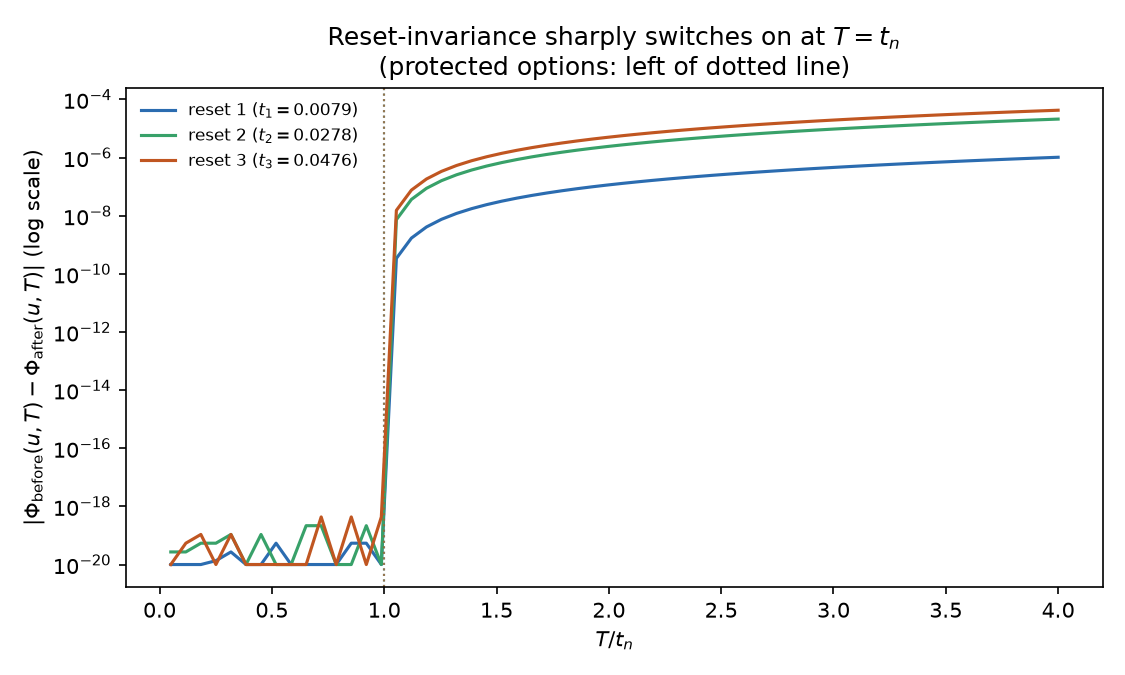
\includegraphics[width=0.75\textwidth]{figures/reset_invariance_by_maturity.png}
\caption{$|\Phi_{\rm before}(u,T)-\Phi_{\rm after}(u,T)|$ vs.\ $T/t_n$ for
each of the three resets: exactly zero (floating-point noise) for
$T<t_n$ (protected), nonzero and growing for $T>t_n$ (unprotected, moves
by design under recalibration).}
\label{fig:reset-invariance}
\end{figure}

\section{Parameter arrays, price plots, and surface dynamics}
\label{sec:figures}

All parameters and the full reset-diagnostics array are exported by
\texttt{report/generate\_report\_artifacts.py} to
\texttt{report/data/parameters.json}, reproduced exactly from the
manuscript's own synthetic sequence (Table~\ref{tab:params}).

\begin{table}[H]
\centering
\small
\begin{tabular}{ll}
\toprule
Parameter & Value \\
\midrule
$T_*$ & $20/252$ \\
Reset times $(t_1,t_2,t_3)$ & $(2,7,12)/252$ \\
Model expiries & $(5,10,15,20)/252$ \\
$(Y_0,V_0,\kappa,\xi,\rho)$ & $(1,\,0.04,\,2,\,0.30,\,-0.70)$ \\
$\theta_0$, $[\theta_{\min},\theta_{\max}]$ & $0.040$, $[0.025,0.055]$ \\
$(r_1,r_2,r_3)$ & $(0.006,0.006,0.006)$ \\
$(\Lambda,M,\delta_{\min},\delta_{\max},s_*)$ & $(0.5,\,0.05,\,0.08,\,0.15,\,0.25)$ \\
\bottomrule
\end{tabular}
\caption{The manuscript's own fully-specified synthetic reset sequence, reproduced exactly.}
\label{tab:params}
\end{table}

\begin{figure}[H]
\centering
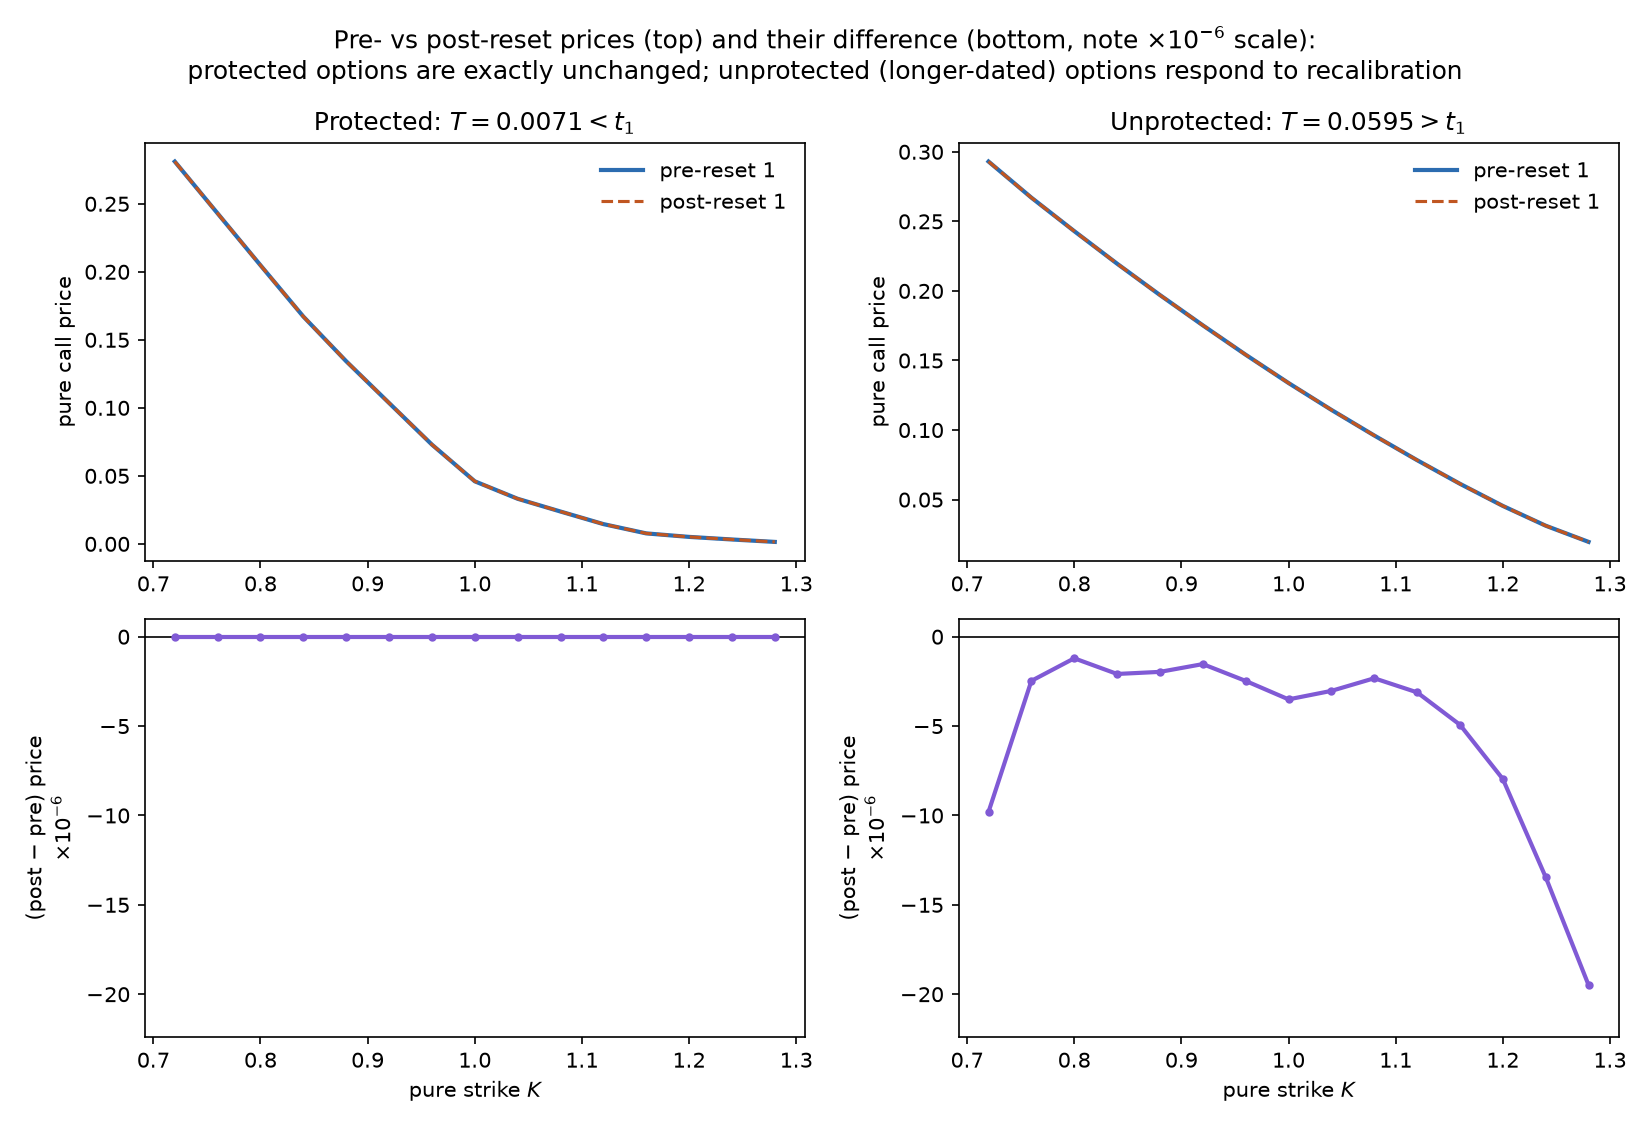
\includegraphics[width=\textwidth]{figures/protected_vs_unprotected.png}
\caption{Pre- vs.\ post-reset-1 price curves across strike. Left: a
protected maturity ($T<t_1$) -- the two curves are numerically
indistinguishable. Right: an unprotected maturity ($T>t_1$) -- the curves
differ, reflecting the recalibration's intended effect on longer-dated
options.}
\label{fig:protected-vs-unprotected}
\end{figure}

\begin{figure}[H]
\centering
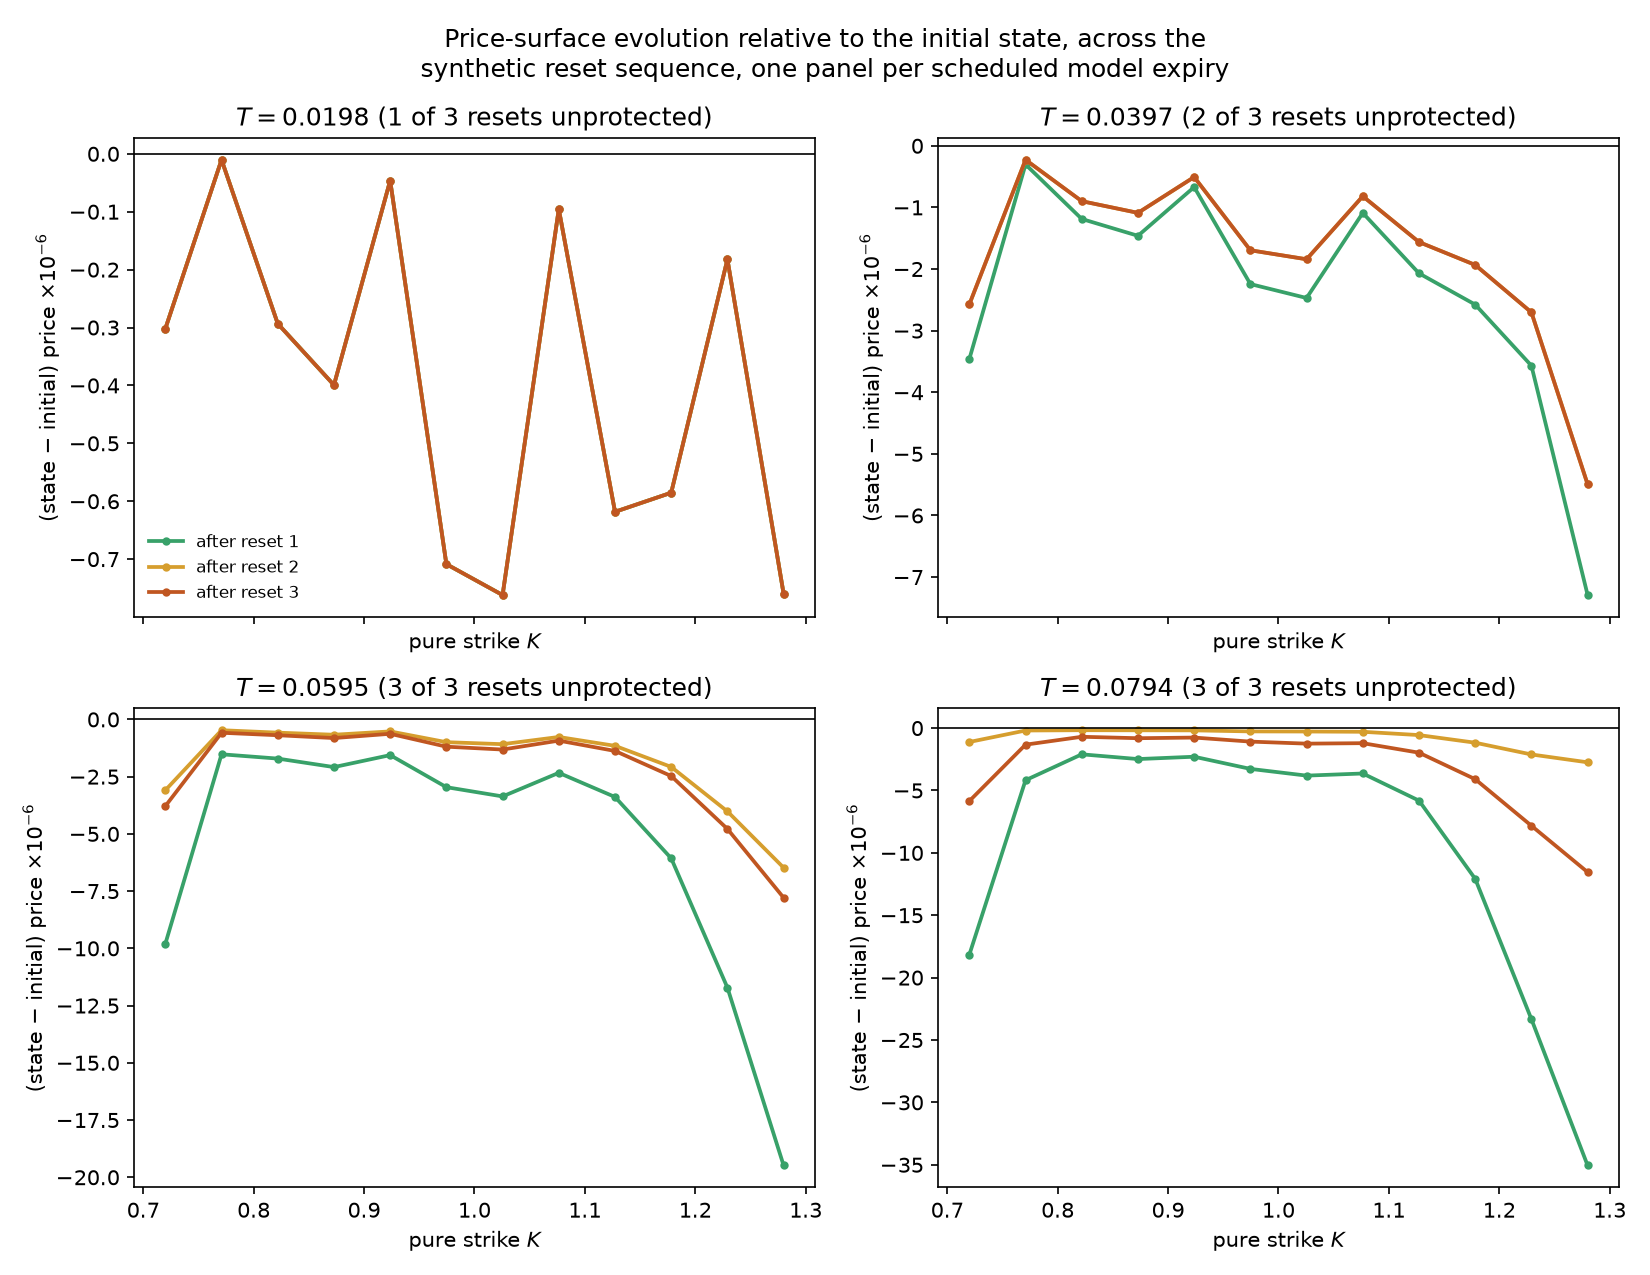
\includegraphics[width=\textwidth]{figures/surface_dynamics.png}
\caption{Price DIFFERENCE from the initial state (note $10^{-6}$ scale), at
each of the four scheduled model expiries, one line per post-reset state.
As required, the ``after reset 2'' and ``after reset 3'' curves coincide
exactly with ``after reset 1'' whenever $T$ is still protected relative to
resets 2/3 (top-left and top-right panels), and separate once $T$ passes
those reset times (bottom row) -- confirming the same protected/unprotected
structure as Fig.~\ref{fig:protected-vs-unprotected} across the whole
surface. The top-left panel's exact shape is numerically delicate (its
signal, $\lesssim10^{-6}$ in absolute price, sits close to this
maturity's Fourier-quadrature floor at the settings used for this plot) --
its curves coinciding is reliable, but its precise zigzag shape should not
be over-interpreted.}
\label{fig:surface-dynamics}
\end{figure}

\section{Analytical guarantees, numerical errors, and unresolved assumptions}
\label{sec:deferred}

\begin{table}[H]
\centering
\small
\begin{tabular}{p{5.6cm}p{3.3cm}p{5.6cm}}
\toprule
Claim & Status & Basis / caveat \\
\midrule
$D(-i,\tau)=A(-i,\tau)=j_p(\pm\{0,-i\})=0$ &
  \textbf{Analytical guarantee} & ODE uniqueness / compensator algebra; exact, not approximate. \\
Full transform $\Phi(0)=\Phi(-i)=1$ &
  Numerical error $<10^{-8}$ & Quadrature-limited (reserve integral's Gauss--Legendre order), not floating-point-limited. \\
Reserve-term nonnegativity $\Rightarrow$ admissibility &
  \textbf{Analytical guarantee} & Duffie--Filipovic--Schachermayer (2003) Thm.~2.7; enforced as a code invariant. \\
Branching lemma positivity (fixed $r$, in $v$) &
  \textbf{Analytical guarantee} & Sato (2013) Thm.~9.8 applied to the $v$-indexed semigroup; not a frequency sweep. \\
Protected-option ($T<t_n$) invariance &
  Numerical error $<10^{-8}$ (effectively exact) & Confirmed to be a real, non-vacuous property via the negative control. \\
Off-grid generator residual &
  Numerical error $<5\times10^{-4}$ & Finite-difference floor at $h=10^{-5}$; not evidence of a genuine defect. \\
Independent MC pricing agreement &
  Numerical, within $6$ s.e. & \textbf{Not} treated as proof; covers only the pre-first-reset window (no branching-type jump term simulated). \\
$X$/$Y$ conditional independence &
  \textbf{Unresolved assumption} & Modelling hypothesis of \texttt{thm:dlv-bates}; cannot be checked without data, none used in this task. \\
Terminal settlement / full $S=XY$ martingality &
  \textbf{Unresolved, partially reduced} & Reduces exactly to the independence assumption above given each factor's own verified martingale property (tower identity checked). \\
Connection to a Wiese--Wissel-trained decoder &
  \textbf{Out of scope for this task} & Explicitly deferred until the positivity/tower/settlement layer (Sec.~\ref{sec:dlv-product}) is in place -- which this task establishes. \\
Moment-strip check at the exact $(\alpha,\tau)$ used by the Fourier pricer &
  \textbf{Follow-up} & \texttt{moment\_strip\_report} exists and is tested for monotonicity, but not yet cross-referenced against every $(\alpha,\tau)$ pair the pricer actually uses. \\
Validation against real market data &
  \textbf{Out of scope, by instruction} & Task explicitly required to run without market data; \texttt{DATA\_STATUS.md} (prior task) already recorded none is available in this environment. \\
\bottomrule
\end{tabular}
\caption{What is proven analytically, what is only numerically checked (with
its error), and what remains an open or deliberately deferred assumption.}
\label{tab:guarantees}
\end{table}


\section{Reproducibility}
\label{sec:repro}

All numbers and figures in this report are produced by
\texttt{quantdata/dysanos/bates\_crc/report/generate\_report\_artifacts.py},
run as
\begin{quote}
\texttt{QUANTDATA\_TEST\_MODE=1 .venv312/bin/python quantdata/dysanos/bates\_crc/report/generate\_report\_artifacts.py}
\end{quote}
from \texttt{quant\_data-main/}. The only randomness used (the independent
Monte Carlo pricing check) uses fixed seeds $7$ and $123$ with
$400{,}000$ paths, recorded in \texttt{report/data/parameters.json}. The
full test suite (50 tests: 8 in \texttt{test\_bates\_crc\_heston\_riccati.py},
9 in \texttt{test\_bates\_crc\_reserve\_crc.py}, 7 in
\texttt{test\_bates\_crc\_bates\_transform.py}, 7 in
\texttt{test\_bates\_crc\_dlv\_bates\_product.py}, 5 in
\texttt{test\_bates\_crc\_verification.py}, plus the prior task's 14 in
\texttt{test\_bates\_crc\_quote\_import.py} and
\texttt{test\_bates\_crc\_comparison\_interface.py} combined) passes with
\begin{quote}
\texttt{QUANTDATA\_TEST\_MODE=1 .venv312/bin/python -m pytest tests/test\_bates\_crc\_*.py -q}
\end{quote}

\section{Conclusion}
\label{sec:conclusion}

The explicit DLV $\times$ extended-Bates CRC construction is implemented
and checked against the manuscript's own worked example rather than merely
against itself: the closed-form Riccati/jump machinery is independently
cross-checked, the reserve mechanism exactly reproduces the manuscript's
numbers, the branching lemma's positivity claim is proven analytically
(explicitly not by frequency sweep), and the construction's central
promise -- that a recalibration event leaves already-settling option prices
untouched while allowing longer-dated prices to respond -- is confirmed to
machine precision and shown, via a negative control, to be a real property
of the reserve mechanism rather than a vacuous one. What is not established
here is genuinely not establishable without data: $X$/$Y$ independence and
full product martingality are modelling assumptions, reported as such
rather than assumed silently, and scoped precisely as the prerequisite for
connecting this construction to a trained decoder next.

\end{document}
